%------------------------------------------------------------
\title[12 - 递归 III]
{12 - 递归 III}

\subtitle{C++ 程序设计进阶}

\author[Beiyu Li]
{Beiyu Li\\
\texttt{<sysulby@gmail.com>}}

% \institute[SOJ]
% {Sicily Online Judge}

\date[\today]
{\number\year 年 \number\month 月 \number\day 日}
%------------------------------------------------------------


\begin{document}

\author[sysulby]
{SOJ 信息学竞赛教练组}

\begin{frame}
    \titlepage
\end{frame}
\setcounter{framenumber}{0} % 标题页不编号


\section{复习回顾}

%------------------------------------------------------------
\begin{frame}[fragile]
    \frametitle{递归}

    \begin{itemize}
        \item 将原问题分解为一个或多个性质相同、规模更小的子问题
        \begin{itemize}
            \item 如何找到子问题是什么?
                \begin{itemize}
                    \item 根据解决问题时需要重复执行的操作或功能
                \end{itemize}
            \item 根据原问题和子问题的相同性质,给递归函数下定义
            \item 子问题与原问题性质相同,调用函数自身解决(自我调用)
            \item 解决子问题后,经过组合/操作形成原问题的答案
            \item 最简子问题直接解答,无需分解(结束条件)
       \end{itemize}
    \end{itemize}
    
\end{frame}
%------------------------------------------------------------


\section{一维分形问题}

%------------------------------------------------------------
\begin{frame}[fragile]
    \frametitle{分形}
    
    \begin{columns}
        \column{.65\textwidth}
        \begin{itemize}
            \item 分形指在不同尺度上都有相似性的图形
            \begin{itemize}
                \item 例如大自然中的闪电
            \end{itemize}
    
            \item 本节课中的分形问题
            \begin{itemize}
                \item 对一维数组不同大小的区域递归进行相同处理的问题称为一维分形问题
                \item 对二维数组不同大小的区域递归进行相同处理的问题称为一维分形问题
            \end{itemize}
        \end{itemize}

        \column{.35\textwidth}
        \begin{figure}
            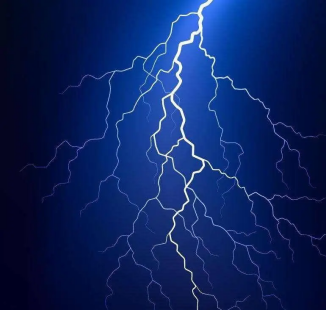
\includegraphics[width=.66\textwidth]{ch24/lightning.png}
        \end{figure}
        
    \end{columns}
\end{frame}
%------------------------------------------------------------


%------------------------------------------------------------
\begin{frame}[fragile]
    \frametitle{例 12.1:无限翻转}
    \only<1> {
        \begin{exampleblock}{编程题}
            \begin{itemize}
                \item 小明和小红为了在上课时间偷偷传字条,想到了一招绝妙的加密方法: \\
                    \begin{itemize}
                        \item 使用英文对话,并且省去空格和标点符号
                        \item 保证长度是 $2$ 的幂 (长度不超过 $2^{10}$)
                        \item 先把英文整体进行左右翻转,然后把这段话分成均匀的前后两半,再对每段分别进行左右翻转,然后再把每段均分为两半,重复上述操作,直到每段话的长度为 $1$
                    \end{itemize}
                    他们想的加密方法绝佳,因为加密过程和解密过程是完全一样的。现小明收到一段密文,请你帮忙解密。
            \end{itemize}
            
            \begin{columns}
                \column{.01\textwidth}

                \column{.49\textwidth}
                \begin{itemize}
                \item 样例输入
    
                    \lstinline|yeuolivo|     
                \end{itemize}

                \column{.5\textwidth}
                \begin{itemize}
                \item 样例输出
                
                    \lstinline|iloveyou| 
                \end{itemize}
            \end{columns}

        \end{exampleblock}
    }
    \only<2>{
        \begin{figure}
            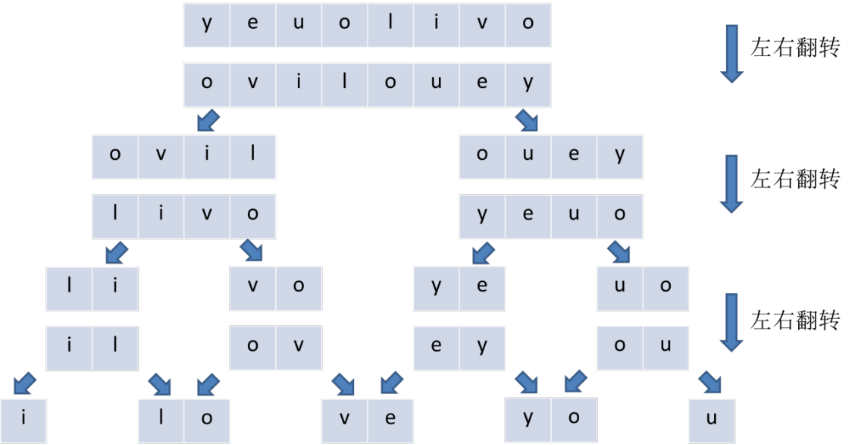
\includegraphics[width=.9\textwidth]{ch24/reverse.png}
        \end{figure}
    }
    \only<3>{
        \begin{itemize}
            \item 原问题:对一个字符串 $s$ 进行“无限翻转”,得到解密结果
                \begin{itemize}
                    \item 将 $s$ 左右翻转后,均分成两个字符串 $s1$ 和 $s2$,分别进行“无限翻转”,得到结果后拼接起来得到 $s$ 的解密结果
                \end{itemize}

            \item 重复的功能:对一个字符串“无限翻转”,得到解密结果
            \item 子问题:对 $s1$ 和 $s2$ 分别进行“无限翻转”,得到解密结果
            \item 下定义:函数 \lstinline|decode(s)| 功能为对字符串 $s$ 进行“无限翻转”,返回解密结果

        \end{itemize}
    }

    \only<4-5>{
        \begin{itemize}
            \item \lstinline|decode(s)| 的实现
            \lstinputlisting[basicstyle=\ttfamily\scriptsize,language=C++,name=decode]{ch24/decode.cc}
            \item<5> 如何实现这两部分?
        \end{itemize}

        \begin{tikzpicture}[remember picture,overlay]
            \only<5>{\redbox{decode}{6}{3}{7}{22}; \redbox{decode}{8}{3}{10}{44};}
        \end{tikzpicture}
    }
    \only<6-10>{
        \begin{itemize}
            \item 左右翻转字符串 $s$
            \only<6> {
                \begin{tikzpicture}
                [nodes in empty cells, nodes={minimum width=1.3cm, minimum height=.7cm}, row sep=-\pgflinewidth, column sep=-\pgflinewidth]
                    \matrix(a) [matrix of nodes, ampersand replacement=\&, nodes={draw, anchor=center}]{
                        \lstinline|a| \& \lstinline|b| \& \lstinline|c| \& \lstinline|d| \& \lstinline|e| \& \lstinline|f| \\
                    };
                \end{tikzpicture}
            }
            \only<7,10> {
                \begin{tikzpicture}
                [nodes in empty cells, nodes={minimum width=1.3cm, minimum height=.7cm}, row sep=-\pgflinewidth, column sep=-\pgflinewidth]
                    \matrix(a) [matrix of nodes, ampersand replacement=\&, column 1/.style={nodes={draw,fill=codegreen!50}}, column 6/.style={nodes={draw,fill=codegreen!50}}, nodes={draw, anchor=center}]{
                        \lstinline|f| \& \lstinline|b| \& \lstinline|c| \& \lstinline|d| \& \lstinline|e| \& \lstinline|a| \\
                    };
                \end{tikzpicture}
            }
            \only<8> {
                \begin{tikzpicture}
                [nodes in empty cells, nodes={minimum width=1.3cm, minimum height=.7cm}, row sep=-\pgflinewidth, column sep=-\pgflinewidth]
                    \matrix(a) [matrix of nodes, ampersand replacement=\&, column 2/.style={nodes={draw,fill=codegreen!50}}, column 5/.style={nodes={draw,fill=codegreen!50}}, nodes={draw, anchor=center}]{
                        \lstinline|f| \& \lstinline|e| \& \lstinline|c| \& \lstinline|d| \& \lstinline|b| \& \lstinline|a| \\
                    };
                \end{tikzpicture}
            }
            
            \only<9> {
                \begin{tikzpicture}
                [nodes in empty cells, nodes={minimum width=1.3cm, minimum height=.7cm}, row sep=-\pgflinewidth, column sep=-\pgflinewidth]
                    \matrix(a) [matrix of nodes, ampersand replacement=\&, column 3/.style={nodes={draw,fill=codegreen!50}}, column 4/.style={nodes={draw,fill=codegreen!50}}, nodes={draw, anchor=center}]{
                        \lstinline|f| \& \lstinline|e| \& \lstinline|d| \& \lstinline|c| \& \lstinline|b| \& \lstinline|a| \\
                    };
                \end{tikzpicture}
            }
            \only<10>{\lstinputlisting[basicstyle=\ttfamily\scriptsize,language=C++,name=reverse]{ch24/reverse.cc}}
            
        \end{itemize}
    }
    \only<11-14>{
        \begin{itemize}
            \item 截取字符串 $s$ 前后两半
            \item \lstinline|substr| 的用法?
            \begin{itemize}
                \item 第一个参数为起始下标,第二个参数为子串长度
                \item<12-> 前后两半字符串的长度固定为 \lstinline|s.size()/2|
                \item<12-> 前后两半字符串的起始下标是多少?
            \end{itemize}
            \uncover<13->{
                \begin{figure}
                    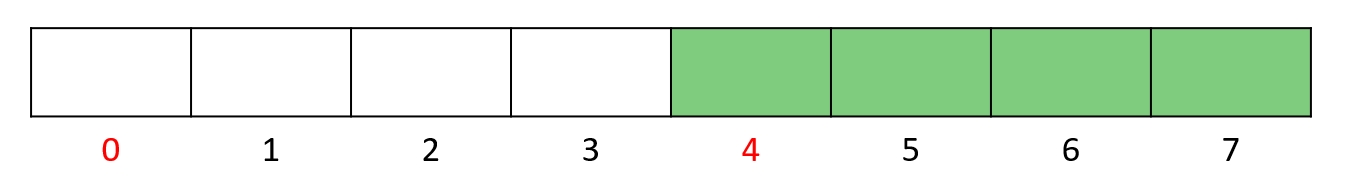
\includegraphics[width=.8\textwidth]{ch24/divide2_beginIndex.png}
                \end{figure}
            }
            \only<14>{
                \lstinputlisting[basicstyle=\ttfamily\scriptsize,language=C++,name=substr]{ch24/substr.cc}
            }
        \end{itemize}
    }
    \only<15>{
        \lstinputlisting[basicstyle=\ttfamily\scriptsize,language=C++,name=InfiniteReverse1]{ch24/InfiniteReverse1.cc}
    }
    \only<16>{
        \lstinputlisting[basicstyle=\ttfamily\scriptsize,language=C++,name=decode_fun]{ch24/decode_fun.cc} 
    
        \begin{itemize}
            \item<16> 每次调用 \lstinline|decode()| ,都会声明一个字符串变量 $s$,并把实参赋值给形参
            \item<16> 多次进行字符串的声明、截取子串、赋值操作,影响代码效率
        \end{itemize}
    }

\end{frame}
%------------------------------------------------------------

%------------------------------------------------------------
\begin{frame}[fragile]
    \frametitle{讨论}

    \begin{block}{}
        \vspace{.5cm}
        \begin{center}
            {\Large 一维分形问题的其他写法}
        \end{center}
        \vspace{.5cm}
    \end{block}
\end{frame}
%------------------------------------------------------------

%------------------------------------------------------------
\begin{frame}[fragile]
    \frametitle{实现方法的改进}
    \begin{itemize}
        \item 在原字符串上进行处理即可,无需截取子串处理后再拼接起来
        \item 如何表示当前处理的是原字符串的哪段区域?
        \begin{itemize}
            \item<2-> 使用两个参数 $L$ 和 $R$,表示当前处理的是字符串 $s$ 下标 $L \sim R$ 的区域
            \item<3-> 使用两个参数 $L$ 和 $len$,表示当前处理的是字符串 $s$ 从下标 $L$ 开始,长度 $len$ 的区域
        \end{itemize}
    \end{itemize}
    \only<1>{
        \begin{figure}
            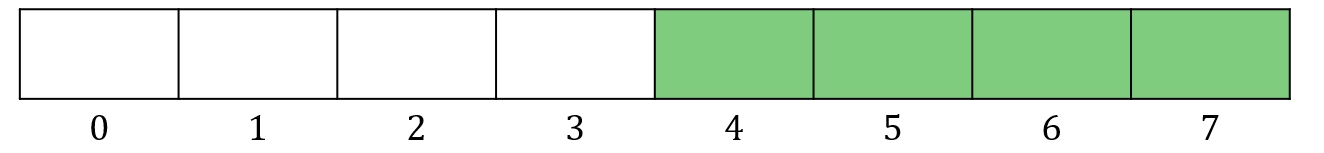
\includegraphics[width=.8\textwidth]{ch24/range.png}
        \end{figure}
    }
    \only<2>{
        \begin{figure}
            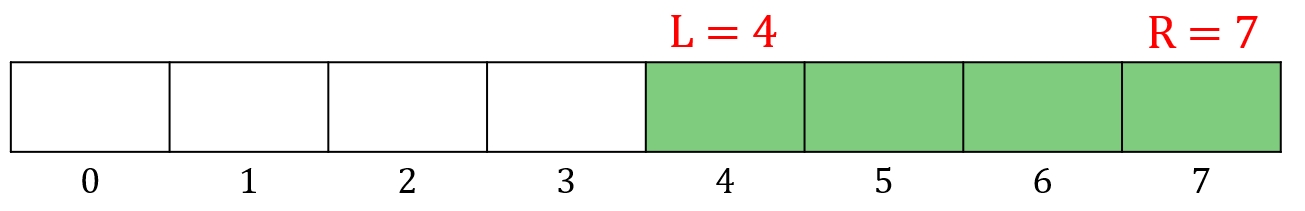
\includegraphics[width=.8\textwidth]{ch24/range_1.png}
        \end{figure}
    }
    \only<3>{
        \begin{figure}
            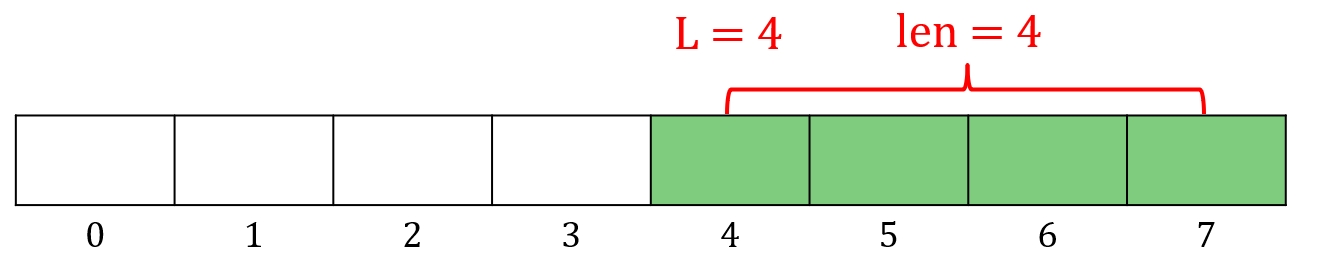
\includegraphics[width=.8\textwidth]{ch24/range_2.png}
        \end{figure}
    }
\end{frame}
%------------------------------------------------------------

%------------------------------------------------------------
\begin{frame}[fragile]
    \frametitle{L、R、len 的关系}
    \begin{figure}
        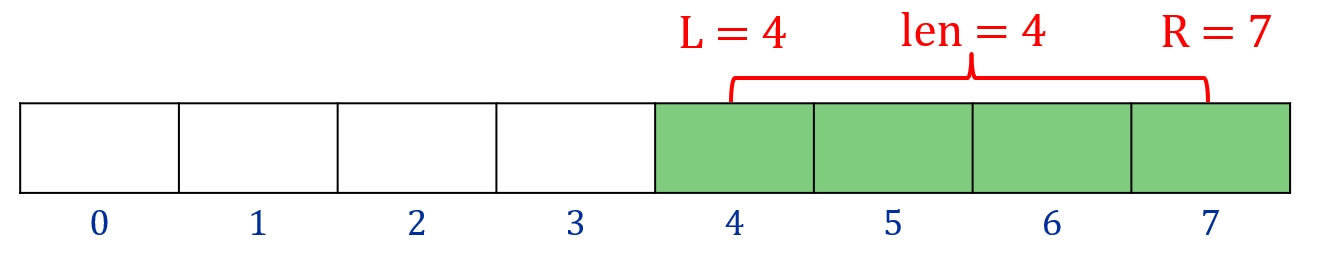
\includegraphics[width=.8\textwidth]{ch24/range_3.png}
    \end{figure}
    \only<1>{
        \begin{itemize}
            \item \lstinline|R = L + len – 1|
            \item \lstinline|len = ?|
            \item \lstinline|L = ?|
        \end{itemize}
    }
    \only<2-3>{
        \begin{itemize}
            \item \lstinline|R = L + len – 1|
            \item \lstinline|len = R - L + 1|
            \item \lstinline|L = R - len + 1|
            \item<3> 易错点:\lstinline|L + len| 不是右端点 \lstinline|R|,而是右端点的下一个位置
        \end{itemize}
    }
\end{frame}
%------------------------------------------------------------

%------------------------------------------------------------
\begin{frame}[fragile]
    \frametitle{问题分析}

    \begin{itemize}
        \item 原问题:对一个字符串 $s$ 进行“无限翻转”,得到解密结果
        \begin{itemize}
            \item 在字符串 $s$ 原地进行“无限翻转”,最后字符串 $s$ 就是解密结果
            \item 将 $s$ 左右翻转后,对其左半区域和右半区域分别进行“无限翻转”
        \end{itemize}
        \item 重复的操作:对 $s$ 的一段区域进行“无限翻转”
        \item 子问题:对当前区域的左半区域和右半区域分别进行“无限翻转”
        \item 下定义:函数 \lstinline|decode(L, len)| 功能为对字符串 $s$ 从下标 $L$ 开始,长度为 $len$ 的区域进行“无限翻转”
    \end{itemize}
\end{frame}
%------------------------------------------------------------

%------------------------------------------------------------
\begin{frame}[fragile]
    \frametitle{decode(L, len) 的实现}
    \begin{itemize}[<+->]
        \item 对同一个字符串 $s$ 进行操作,$s$ 声明为全局变量,无需作为参数传递
        \item 字符串 $s$“无限翻转”后就是答案,函数无需返回值
        \item 对从下标 $L$ 开始,长度为 $len$ 的区域进行左右翻转
        \begin{itemize}
            \item 注意右端点为:\lstinline|L + len – 1|
        \end{itemize}
        \item 当前区域的左半区域和右半区域的起始下标、长度分别是多少?
        \begin{itemize}
            \item 左半区域:\lstinline|L, len / 2|
            \item 右半区域:\lstinline|L + len / 2, len / 2|
        \end{itemize}
    \end{itemize}
\end{frame}
%------------------------------------------------------------

%------------------------------------------------------------
\begin{frame}[fragile]
    \frametitle{代码实现}
    \lstinputlisting[basicstyle=\ttfamily\scriptsize,language=C++,name=InfiniteReverse2]{ch24/InfiniteReverse2.cc}
\end{frame}
%------------------------------------------------------------

%------------------------------------------------------------
\begin{frame}[fragile]
    \frametitle{一维分形问题}
    \begin{itemize}
        \item 原问题:对一维数组进行操作
        \item 子问题:对划分出的子区域进行相同操作
        \item 技巧
        \begin{itemize}
            \item 数组声明在全局区,在原数组上进行操作
            \item 使用参数 \lstinline|(L, len)| 或 \lstinline|(L, R)| 来表示当前处理的是哪个区域
            \item 无需将子区域的内容复制到别的数组进行处理
        \end{itemize}
    \end{itemize}

\end{frame}
%------------------------------------------------------------

\section{二维分形问题}

%------------------------------------------------------------
\begin{frame}[fragile]
    \frametitle{例 12.2:赦免战俘}
        \begin{exampleblock}{编程题}
        \only<1>{
            \begin{itemize}
                \item 有 $2^n \times 2^n (n \leq 10)$ 名战俘站成一个正方形方阵等待领主的发落。领主决定按照以下方式赦免一些战俘:\\
                    \begin{itemize}
                    \item 他将正方形矩阵均分为 $4$ 个更小的正方形矩阵,每个小矩阵的边长是原矩阵的一半。
                    \item 其中左上角那一个小矩阵的所有战俘都将得到赦免;剩下 $3$ 个小矩阵中,每一个矩阵继续分为 $4$ 个更小的矩阵,然后通过同样的方式赦免战俘,不断重复此操作直到矩阵无法再分下去为止。
                    \end{itemize}
                输出 $2^n \times 2^n$ 的 $01$ 矩阵,其中 $0$ 表示被赦免的战俘,$1$ 表示未被赦免的战俘
            \end{itemize}
        }
        \only<2>{
            \begin{itemize}
            \item 样例输入

                \lstinline|2|    
            \item 样例输出
            
                \lstinline|0 0 0 1|\\
                \lstinline|0 0 1 1|\\
                \lstinline|0 1 0 1|\\
                \lstinline|1 1 1 1|
            \end{itemize}
    
            \begin{figure}
                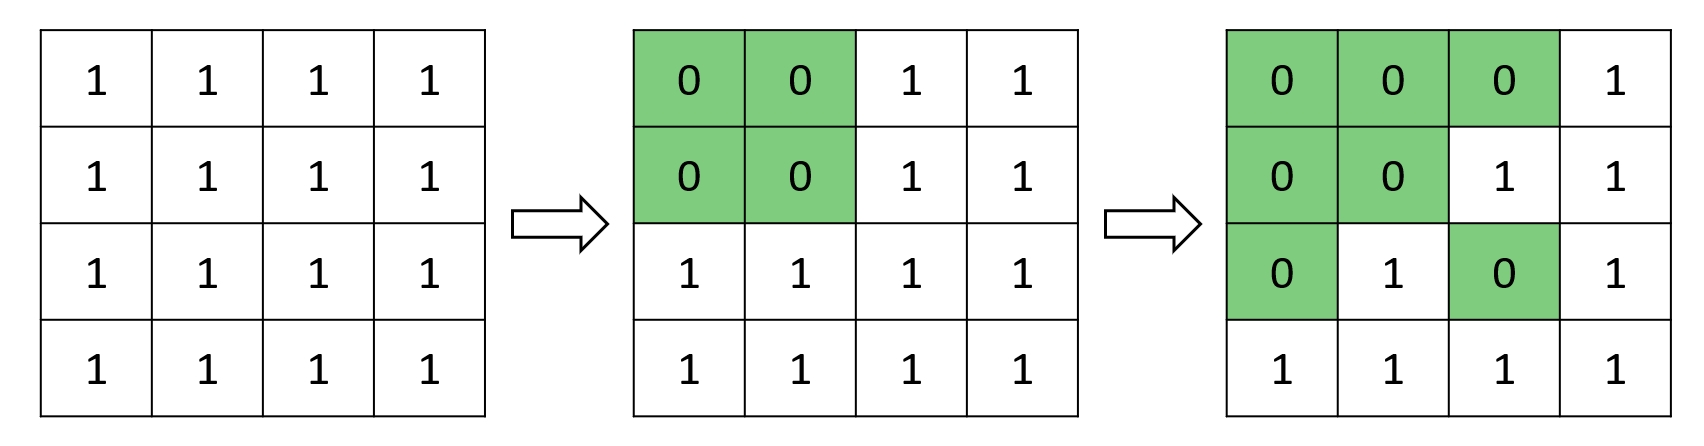
\includegraphics[width=.66\textwidth]{ch24/sm.png}
            \end{figure}
        }

        \end{exampleblock}
\end{frame}
%------------------------------------------------------------


%------------------------------------------------------------
\begin{frame}[fragile]
    \frametitle{问题分析}

    \begin{itemize}
        \item 原问题:对 $2^n \times 2^n$ 的二维区域进行“赦免”操作
        \begin{itemize}
            \item 对左上角的子区域全部赋值为 $0$
            \item 对另外 $3$ 个子区域按照同样的规则进行“赦免”操作
        \end{itemize}
        \item 重复的操作:对某个二维区域进行“赦免”操作
        \item 子问题:对当前区域的右上、左下、右下子区域进行“赦免”操作
        \item 下定义:函数 \lstinline|absolve(二维区域)| 的功能为对当前区域进行“赦免”操作
    \end{itemize}
\end{frame}
%------------------------------------------------------------

%------------------------------------------------------------
\begin{frame}[fragile]
    \frametitle{二维区域的表示}

    \begin{itemize}[<+->]
        \item 一维数组可以用 \lstinline|(L, R)| 或 \lstinline|(L, len)| 的方式表示一段区域,二维数组如何表示一块区域?
        \begin{itemize}
            \item \lstinline|(x1, y1, x2, y2)| 表示左上角在 \lstinline|(x1, y1)|、右下角在 \lstinline|(x2, y2)| 的矩形区域
            \item \lstinline|(x, y, xlen, ylen)| 表示左上角在 \lstinline|(x, y)|,且有 \lstinline|xlen| 行、\lstinline|ylen| 列的矩形区域
            \item 本题每个区域都是正方形,行数 \lstinline|xlen| 与列数 \lstinline|ylen| 相同,可用 \lstinline|(x, y, len)| 表示
        \end{itemize}
    \end{itemize}
    
    \only<1>{
        \begin{figure}
            
\includegraphics[width=.35\textwidth]{ch24/range2.png}
        \end{figure}
    }
    \only<2>{
        \begin{figure}
            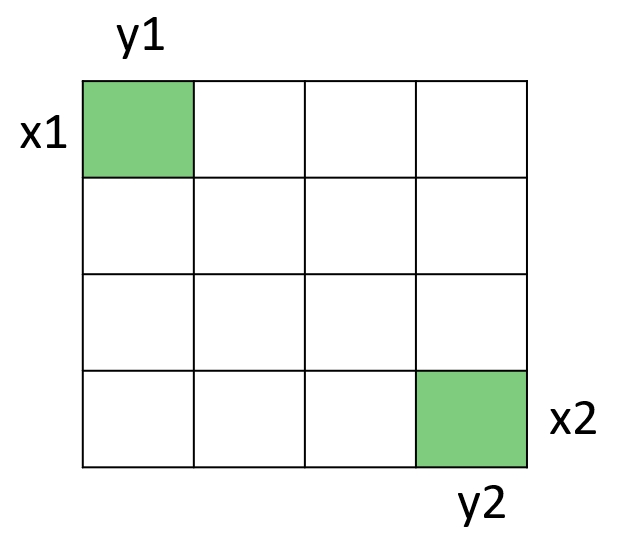
\includegraphics[width=.35\textwidth]{ch24/range2_1.png}
        \end{figure}
    }
    \only<3>{
        \begin{figure}
            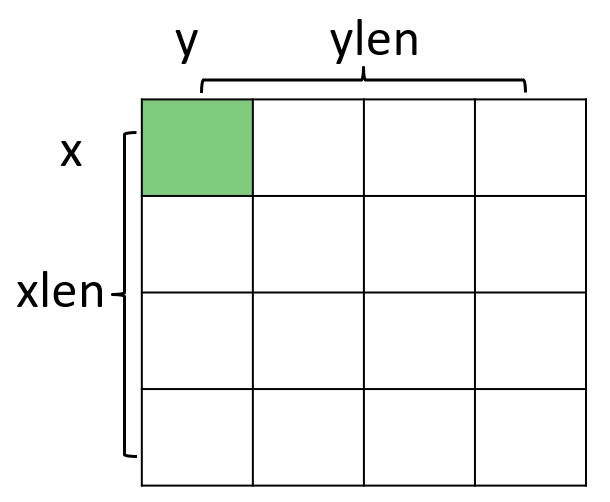
\includegraphics[width=.35\textwidth]{ch24/range2_2.png}
        \end{figure}
    }
    \only<4>{
        \begin{figure}
            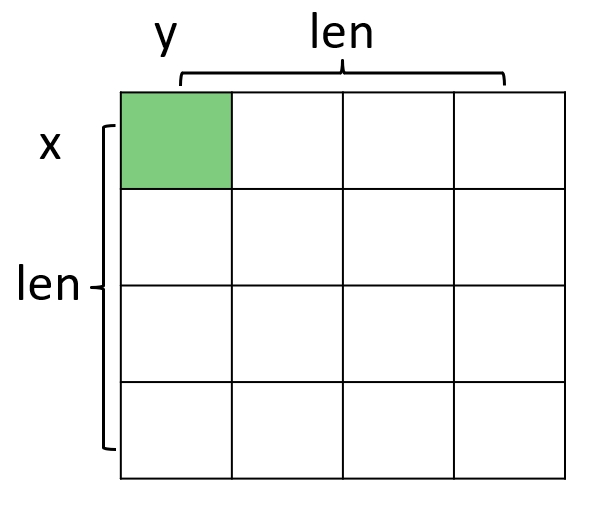
\includegraphics[width=.35\textwidth]{ch24/range2_3.png}
        \end{figure}
    }
\end{frame}
%------------------------------------------------------------

%------------------------------------------------------------
\begin{frame}[fragile]
    \frametitle{子区域位置计算}

    \begin{itemize}[<+->]
        \item 已知左上角位置为 \lstinline|(x, y)|,边长为 $len$ 的区域,分成的 $4$ 个区域的左上角和边长都是多少呢?
        \begin{itemize}
            \item<2-> $4$ 个子区域都是大小相同的正方形,边长均为 \lstinline|len / 2|
            \item<3-> 第一个子区域的左上角位置为 \lstinline|(x, y)|
            \item<4-> 第二个子区域的左上角位置为 \lstinline|(x, y + len / 2)|
            \item<5-> 第三个子区域的左上角位置为 \lstinline|(x + len / 2, y)|
            \item<6-> 第四个子区域的左上角位置为 \lstinline|(x + len / 2, y + len / 2)|
        \end{itemize}
    \end{itemize}
    
    \only<1-2>{
        \begin{figure}
            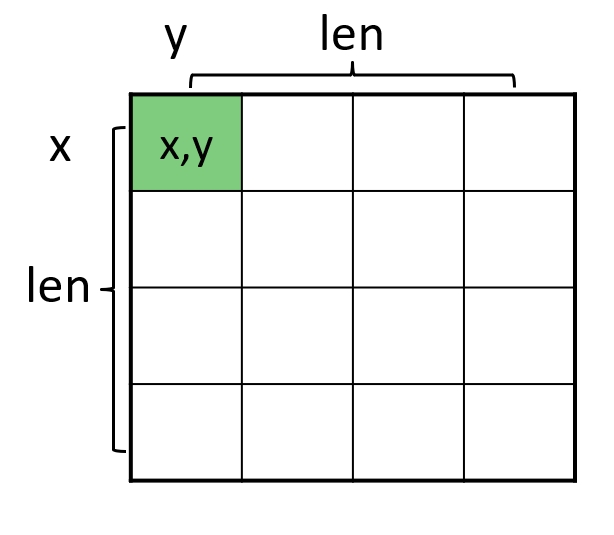
\includegraphics[width=.35\textwidth]{ch24/divide4_1.png}
        \end{figure}
    }
    \only<3>{
        \begin{figure}
            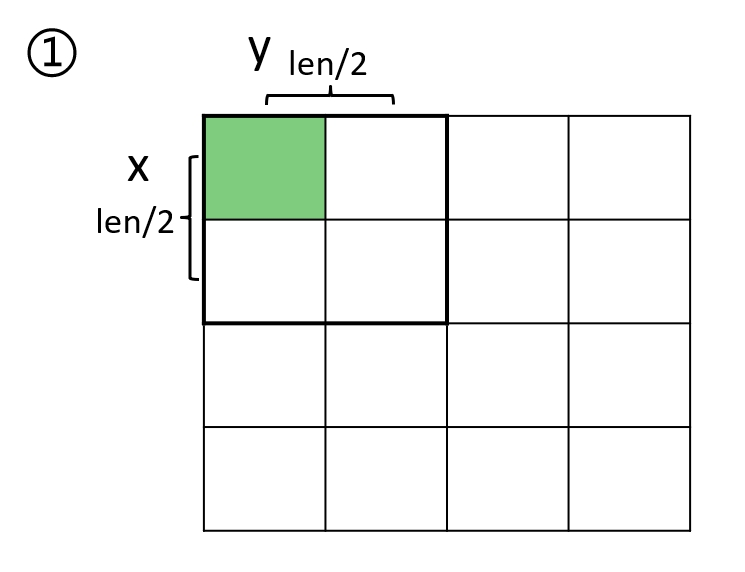
\includegraphics[width=.35\textwidth]{ch24/divide4_2.png}
        \end{figure}
    }
    \only<4>{
        \begin{figure}
            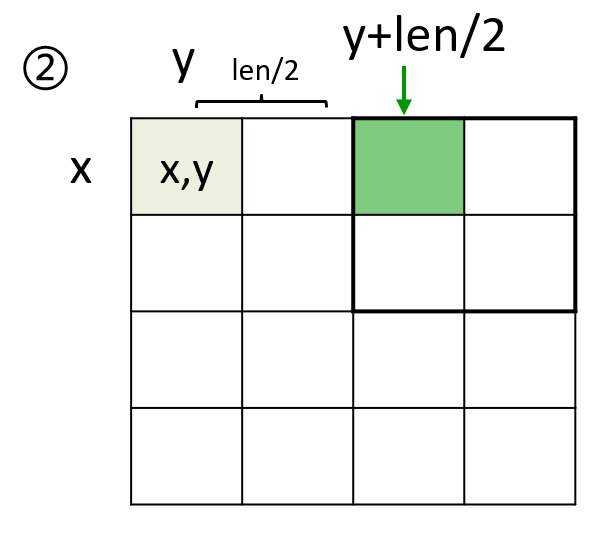
\includegraphics[width=.35\textwidth]{ch24/divide4_3.png}
        \end{figure}
    }
    \only<5>{
        \begin{figure}
            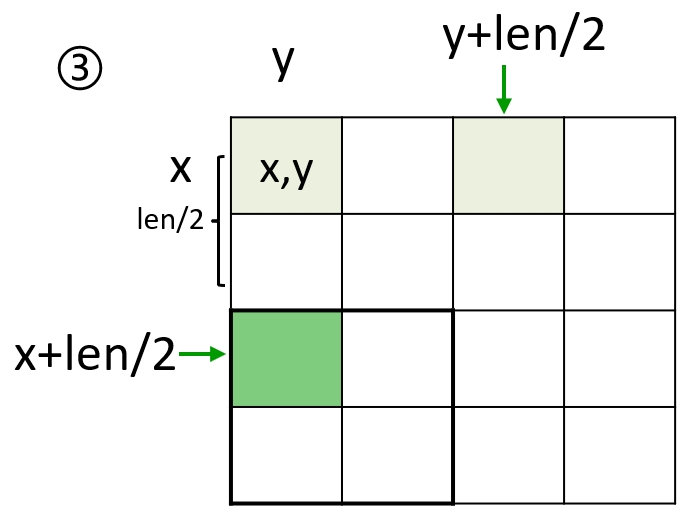
\includegraphics[width=.35\textwidth]{ch24/divide4_4.png}
        \end{figure}
    }
    \only<6>{
        \begin{figure}
            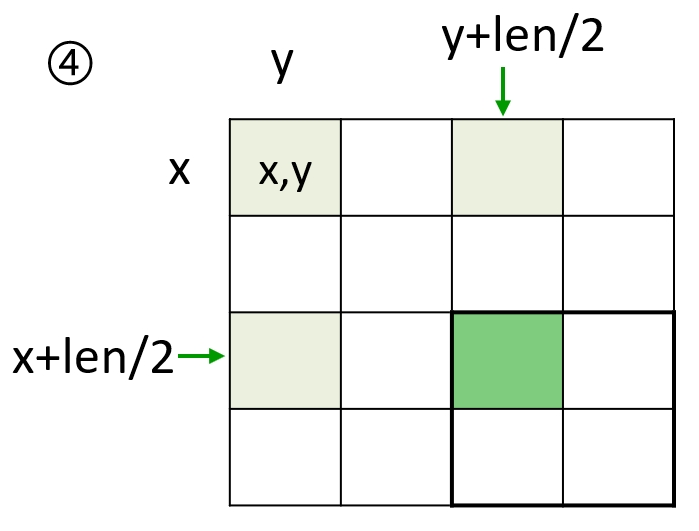
\includegraphics[width=.35\textwidth]{ch24/divide4_5.png}
        \end{figure}
    }
\end{frame}
%------------------------------------------------------------

%------------------------------------------------------------
\begin{frame}[fragile]
    \frametitle{absolve(x, y, len) 的实现}
    \begin{itemize}[<+->]
        \item 功能是对左上角为第 $x$ 行第 $y$ 列,边长为 $len$ 的正方形区域进行“赦免”操作
        \item 左上角子区域全部赋值为 $0$
        \begin{itemize}
            \item 第几行到第几行,第几列到第几列?
            \item 第 $x$ 到 $x + len / 2 - 1$ 行,第 $y$ 到 $y + len / 2 - 1$ 列
        \end{itemize}
        \item 其他三个子区域递归调用函数,进行“赦免”操作
        \item 最简子问题:\lstinline|len == 1| 时,无需操作
    \end{itemize}
\end{frame}
%------------------------------------------------------------

%------------------------------------------------------------
\begin{frame}[fragile]
    \frametitle{代码示例}
    
    \only<1>{
        \lstinputlisting[basicstyle=\ttfamily\scriptsize,language=C++,name=absolve]{ch24/absolve.cc}
    }
    \only<2>{
        \lstinputlisting[basicstyle=\ttfamily\scriptsize,language=C++,name=absolve_main_1]{ch24/absolve_main_1.cc}
    }
    \only<3>{
        \lstinputlisting[basicstyle=\ttfamily\scriptsize,language=C++,name=absolve_main_0]{ch24/absolve_main_0.cc}
        \begin{tikzpicture}[remember picture,overlay]
            \redbox{absolve_main_0}{6}{8}{6}{26};
             \redbox{absolve_main_0}{7}{10}{7}{28};
             \redbox{absolve_main_0}{11}{11}{11}{14};
             \redbox{absolve_main_0}{13}{8}{13}{26};
             \redbox{absolve_main_0}{14}{10}{14}{28};
        \end{tikzpicture}
    }

\end{frame}
%------------------------------------------------------------


\section{总结}

%------------------------------------------------------------
\begin{frame}[fragile]
    \frametitle{递归总结}
    \begin{itemize}
        \item 递归的特点:函数调用自身
        \item 适用问题
        \begin{itemize}
            \item 原问题的求解需要解决一个或多个性质相同、规模更小的子问题
        \end{itemize}
        \item 根据原问题和子问题的相同性质,给递归函数下定义
        \begin{itemize}
            \item 注意函数参数、返回值的含义和类型
            \item 注意递归的终止
        \end{itemize}
        \item 相关的应用
        \begin{itemize}
            \item 数值计算(数列、gcd)
            \item 分裂问题
            \item 分形问题(用参数表示区域、注意子区域的起始位置计算)
        \end{itemize}
    \end{itemize}

\end{frame}
%------------------------------------------------------------

\end{document}